% !TeX spellcheck = de_DE
\documentclass{article} 
%\KOMAoptions{fontsize=12pt, paper=a4}
%\KOMAoptions{DIV=11}
\usepackage[ngerman]{babel}
\def\nummer{1}
\def\datum{29.04.2025}
\def\titel{Ausbreitung von Signalen auf Leitungen}
%TODO: Name, Nummer, Datum	
\title{Versuch \nummer~-  \titel}
\date{\datum}
\usepackage{amsmath, amssymb, amsthm} 
\usepackage{geometry}
\usepackage[utf8]{inputenc}
\usepackage{enumerate}
\usepackage[shortlabels]{enumitem}
\usepackage{authblk}
\usepackage{fancyhdr}
\usepackage{titlesec}

\usepackage{../pakete}
\usepackage{../aufgaben}


\addbibresource{../referenzen.bib}
\geometry{a4paper, left=3cm, right=3cm, top=3cm, bottom=3cm}

\newtheorem{theorem}{Satz}
\newtheorem{lemma}[theorem]{Lemma}
\newtheorem{korollar}{Korollar}[section]
\theoremstyle{definition}
\newtheorem{definition}[theorem]{Definition}
\newtheorem{beispiel}[theorem]{Beispiel}
\newtheorem{satz}[theorem]{Satz}

%\displaystyle \lim_{x \to \infty}



\begin{document}
    \title{Elektronikpraktikum \\ \textbf{Versuch 2: Diodenkennlinien}}
    \author[1]{Carlos Pascua \thanks{s87cpasc@uni-bonn.de}}
    \author[1]{Anna Maróti\thanks{s32amaro@uni-bonn.de}}
    \author[1]{Cornelius Heiming\thanks{s64cheim@uni-bonn.de}}
    \affil[1]{Uni Bonn}
    %\date{\today}
	\pagenumbering{gobble}
    \begin{titlepage}
     \maketitle   
    \end{titlepage}
        
\tableofcontents
\newpage
\pagenumbering{arabic}

\pagestyle{fancy}
\fancyhead[R]{\thepage}
\fancyhead[L]{\leftmark}

% === Einleitung ===
\section{Einleitung}

% === Theorie ====
\section{Theorie}
    \subsection{Halbleiter und Dotierung}
    Halbleiter sind im allgemeinsten Falle Stoffe, die sich unter verschiedenen Umständen wie Leiter oder aber wie Nichtleiter verhalten. Dies liegt an der geringen Anzahl an vorhandenen Ladungsträgern, welche man durch gezielte Verunreinigung des Stoffes (sogennante Dotierung) explizit beeinflussen kann. 

    Konkret verwendet man häufig Kristalle von Elementen mit vier Valenzelektronen (bspw. Silizium oder Germanium), welche mit Elementen der dritten bzw. fünften Hauptgruppe verunreinigt, d.h. dotiert werden. Ersteres liefert einen Mangel an freien Elektronen, um die vervollständigte Kristallstruktur zu erreichen, weshalb diese als p(ositiv)-dotiert gelten. Andersherum sorgen Elemente der fünften Hauptgruppe für einen Elektronenüberschuss, also eine n(egativ)-Dotierung.

    Bringt man nun eine p-Dotierte und eine n-Dotierte Schicht zusammen, können Elektronen übergehen. Dadurch entsteht allerdings eine elektrische Kraft, welches der molekularen Bindungskraft entgegen wirkt, es ergibt sich also ein Gleichgewicht von Kräften. In dem Bereich des Kräftegleichgewichts liegen keine freien Ladungsträger vor, da diese vollständig gebunden sind, d.h. diese Schicht ist nichtleitend. Durch ein äußeres elektrisches Feld (Spannung) kann aber das innere elektrische Feld überlagert werden, was, je nach Richtung der Spannung eine Vergrößerung bzw. Verkleinerung des elektrischen Felds zufolge hat. Ab dem Punkt, an welchem sich äußeres und inneres Feld ausgleichen, liegt keine Grenzschicht mehr vor, die Kombination ist also leitend.  
    \subsection{Diode}
    Eine Diode ist ein elektronisches Bauelement, welches den Strom in genau einer Richtung durchlässt. Man spricht von Durchlass- und Sperrrichtung Diese wird zumeist mit einem Halbleiter, wie oben beschrieben, umgesetzt.
    \begin{figure}[H]
        \centering
        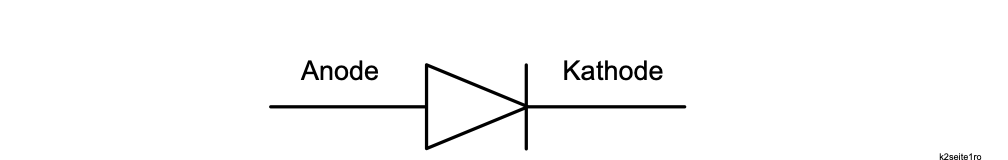
\includegraphics[width=0.8\textwidth]{figs/fig2_1.png}
        \caption{Schaltzeichen Diode\cite{anleitung}}
        \label{fig:Abb2.1}
    \end{figure}

    \subsection{Realität \& Diodenkennlinien}
    In der Realität kann eine Diode die idealisierende Bedingung von Durchlass in einer Richtung und Sperrung in der entgegengesetzten nicht erreichen. In Durchlassrichtung muss zunächst die Grenzschicht mittels eines äußeren Felds überwunden werden, danach verhält sich die Diode wie ein Leiter. In der Sperrichtung kann zunächst stets ein kleiner Strom beobachtet werden, da die freien Ladungsträger der n-dotierten Schicht sich an der Kathode befinden, also einfach abfließen können. Die Elektronen fließen dann durch den Halbleiter nach. Wenn die Spannung in Sperrrichtung groß genug wird, durchbricht die Diode, ist zerstört und leitet den Strom ebenfalls. Dadurch kann man die U-I-Beziehung an einer Diode betrachten - die Diodenkennlinie \ref{fig:Abb2.2}:
    \begin{figure}[H]
        \centering
        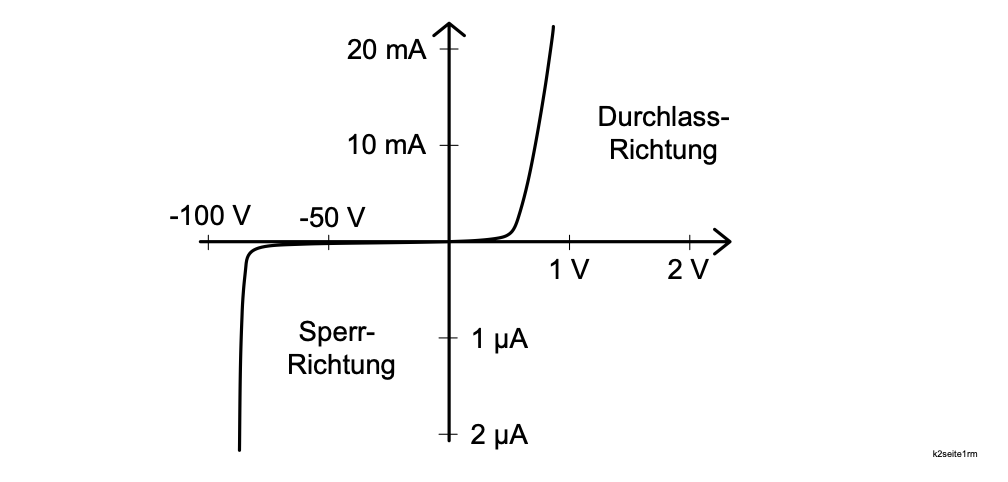
\includegraphics[width=0.8\textwidth]{figs/fig2_2.png}
        \caption{Diodenkennlinie\cite{anleitung}}
        \label{fig:Abb2.2}
    \end{figure}
    \subsection{Gleichrichter}
    Die grundlegende Eigenschaft einer Diode kann verwendet werden, um eine Wechselspannung in eine Gleichspannung umzuwandeln. Am einfachsten geschieht dies durch in-Reihe-Schalten einer Diode, sodass nur Spannungen einer Richtung auftauchen (vgl. \ref{fig:Abb2.4mod} a)). Nachteil daran ist, dass dann mit der Frequenz der Wechselspannnung negative Spannungen, welche durch die Diode annuliert werden, vorliegen. Um dies zu vermeiden, wird ein Zweiweggleichrichter verwendet (vgl. \ref{fig:Abb2.4mod} a)).
    - die Diodenkennlinie \ref{fig:Abb2.2}:
    \begin{figure}[H]
        \centering
        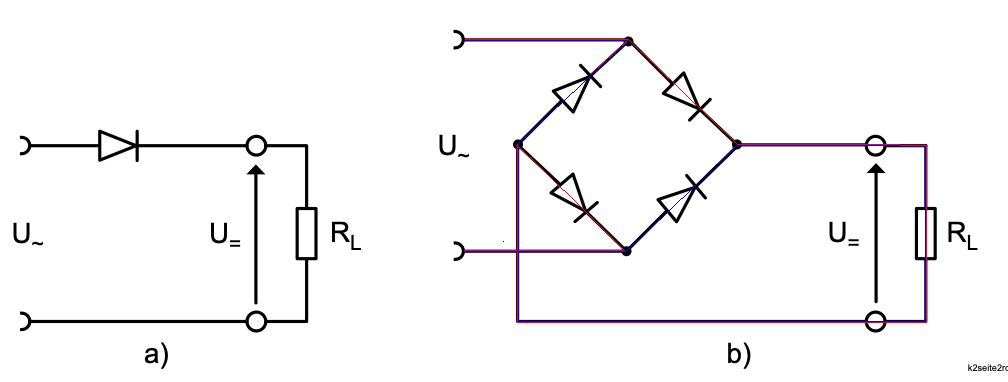
\includegraphics[width=0.8\textwidth]{figs/fig2_4mod.png}
        \caption{Ein- und Zweiweggleichrichter\cite{anleitung}}
        \label{fig:Abb2.4mod}
    \end{figure}
    

    Auch wenn dies die Spannung gleichrichtet, kommen diverse realistische Effekte zu tragen, welche dafür sorgen, dass keine glatte Gleichspannung entsteht, diese Abweichung wird "Brumm" genannt. Um dies nun auch noch auszuglätten wird parallel zum Verbraucher ein Kondensator angelegt.
% === Voraufgaben ===
\section{Voraufgaben}

% == A ==
    \begin{voraufgabe}{Was bestimmt die Dicke der Grenzschicht bei einem p-n-Halbleiter?}
        Die Dicke der Grenzschicht ist abhängig von der Dotierung und dem äußeren elektrischen Feld. Erstere sorgt für die Bereitstellung von Ladungsträgern (Elektronen oder "Löcher"), welche die Grenzschicht bilden und durch das äußere elektrische Feld beeinflusst werden.
    \end{voraufgabe}
% == B ==
    \begin{voraufgabe}{Wie ändert sich die Kapazität einer Diode im Sperrfall mit der angelegten Spannung?}
        Im Sperrfall kann die Diode Modellhaft als Plattenkondensator mit dem Sperrband als Dielektrikum modelliert werden. Für die Dicke des Sperrbands $d$, dessen relative elektische Permeabilität $\epsilon_r$ und die Durchschnittsfläche der Diode $A$ gilt:
        \begin{equation}
            C = \epsilon_0 \epsilon_r \frac{A}{d} \propto \frac{1}{\sqrt{U_\mathrm{ext}}}
            \label{Kapazität einer Diode}
        \end{equation}
    \end{voraufgabe}
    
% == C ==
\begin{voraufgabe}{Skizzieren Sie den Kennlinienverlauf, $I=f(U)$, der Zweipole aus Abb. 2.3 (\ref{fig:Abb2.3}) $(R = \SI{100}{\ohm}; D = \text{Diode})$. Erläutern Sie bei c) und d) den Einfluss der Widerstände.}
    \begin{figure}[H]
        \centering
        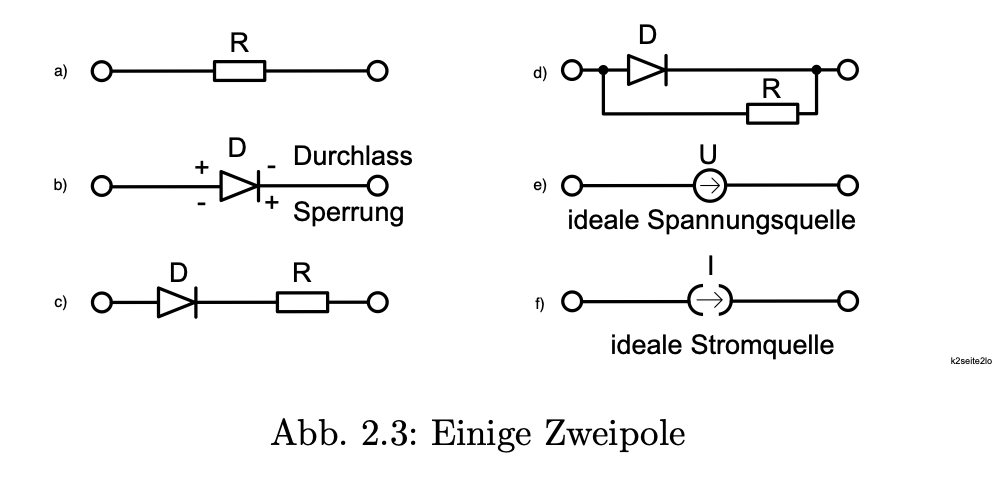
\includegraphics[width=0.8\textwidth]{figs/fig2_3.png}
        \caption{Einige Zweipole\cite{anleitung}}
        \label{fig:Abb2.3}
    \end{figure}
    \begin{figure}[H]
        \centering
        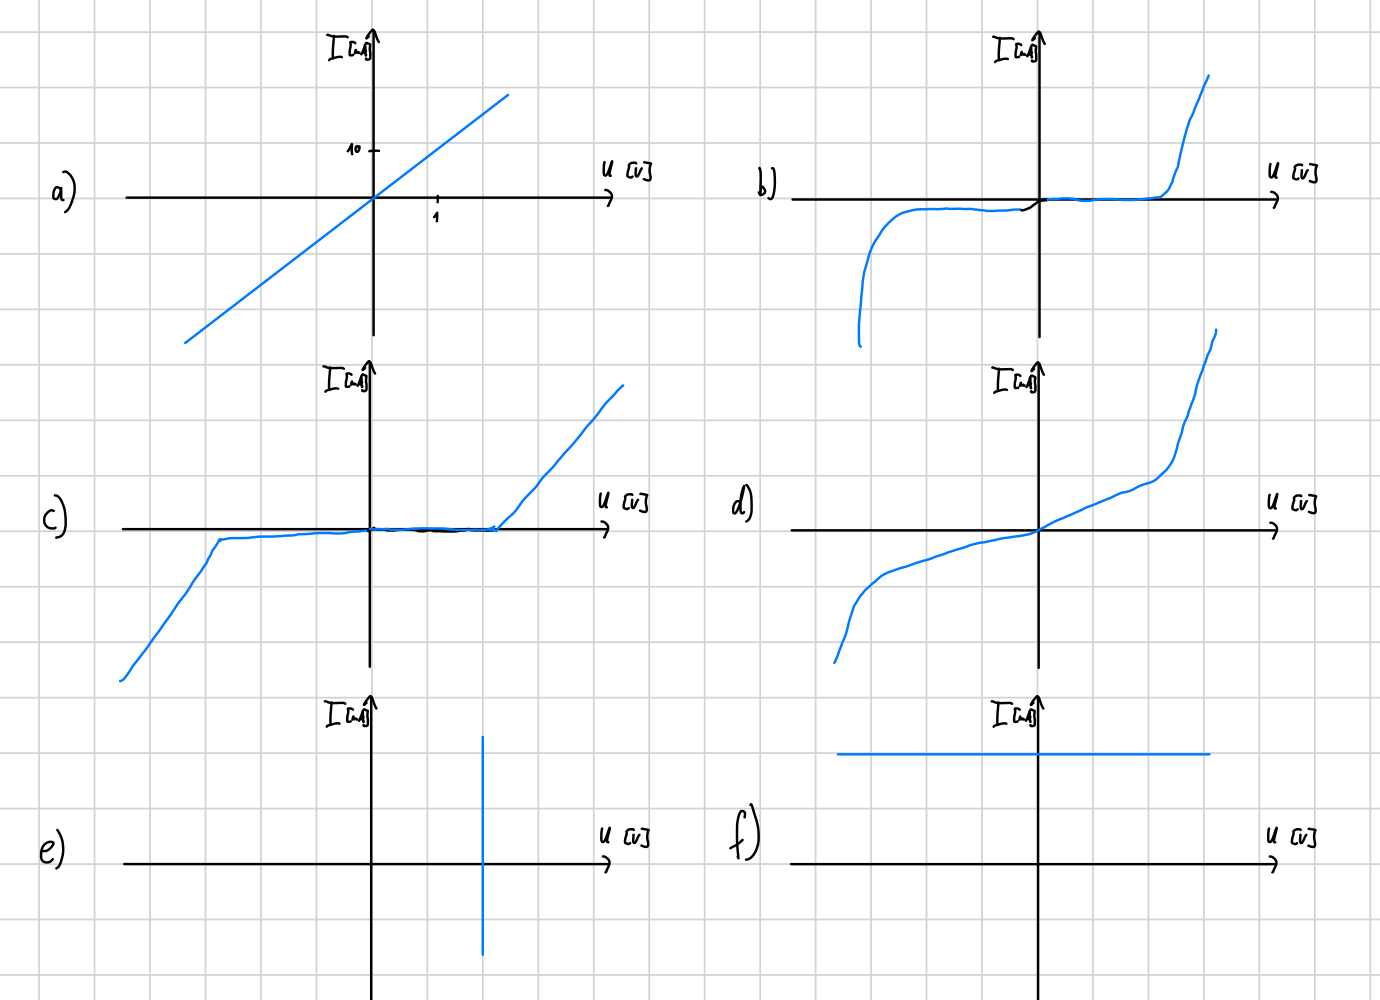
\includegraphics[width=0.8\textwidth]{figs/fig2_C.png}
        \caption{Kennlinienverläufe einiger Zweipole}
        \label{figC}
    \end{figure}
    Bei c) ist der Widerstand hinter der Diode in Reihe geschaltet. Für den Bereich, in dem die Diode keinen Strom durchlässt, ist der Strom $0$, woran auch der Widerstand nichts ändert. Lässt die Diode allerdings Strom durch, so spiegelt sich der lineare Anstieg durch den Widerstand wider.

    Bei d) sind Diode und Widerstand parallel geschaltet. In Sperrrichtung sorgt eine zu hohe Spannung für eine Zerstörung der Diode, wodurch diese zu einem Leiter wird, weshalb der Strom haupsächlich über diese fließt. Bei einer geringen Sperrrichtungsspannung wird die Diode nahezu ignoriert, weshalb ein linearer Anstieg vorliegt. Wird die Diode leitend, handelt es sich um parallelgeschaltete Widerstände, was einen höheren Strom ermöglicht.

\end{voraufgabe}
% == D ==
\begin{voraufgabe}{Skizzieren Sie den zeitlichen Verlauf der Ausgangsspannungen der Schaltungen in Abb. 2.4 (\ref{fig:Abb2.4}) (a) und (b), wenn die Eingangsspannung eine weit über der Durchlassspannung der Dioden liegende Sinusspannung ist.}
    \begin{figure}[H]
        \centering
        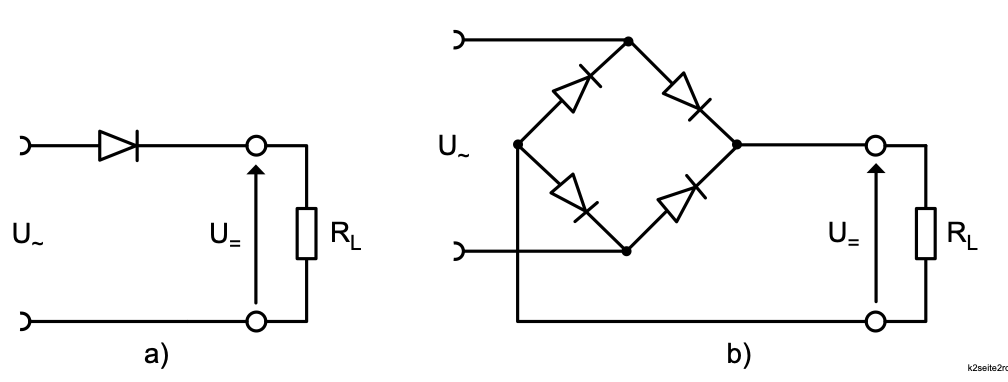
\includegraphics[width=0.8\textwidth]{figs/fig2_4.png}
        \caption{Ein- und Zweiweggleichrichter\cite{anleitung}}
        \label{fig:Abb2.4}
    \end{figure}
    \begin{figure}[H]
        \centering
        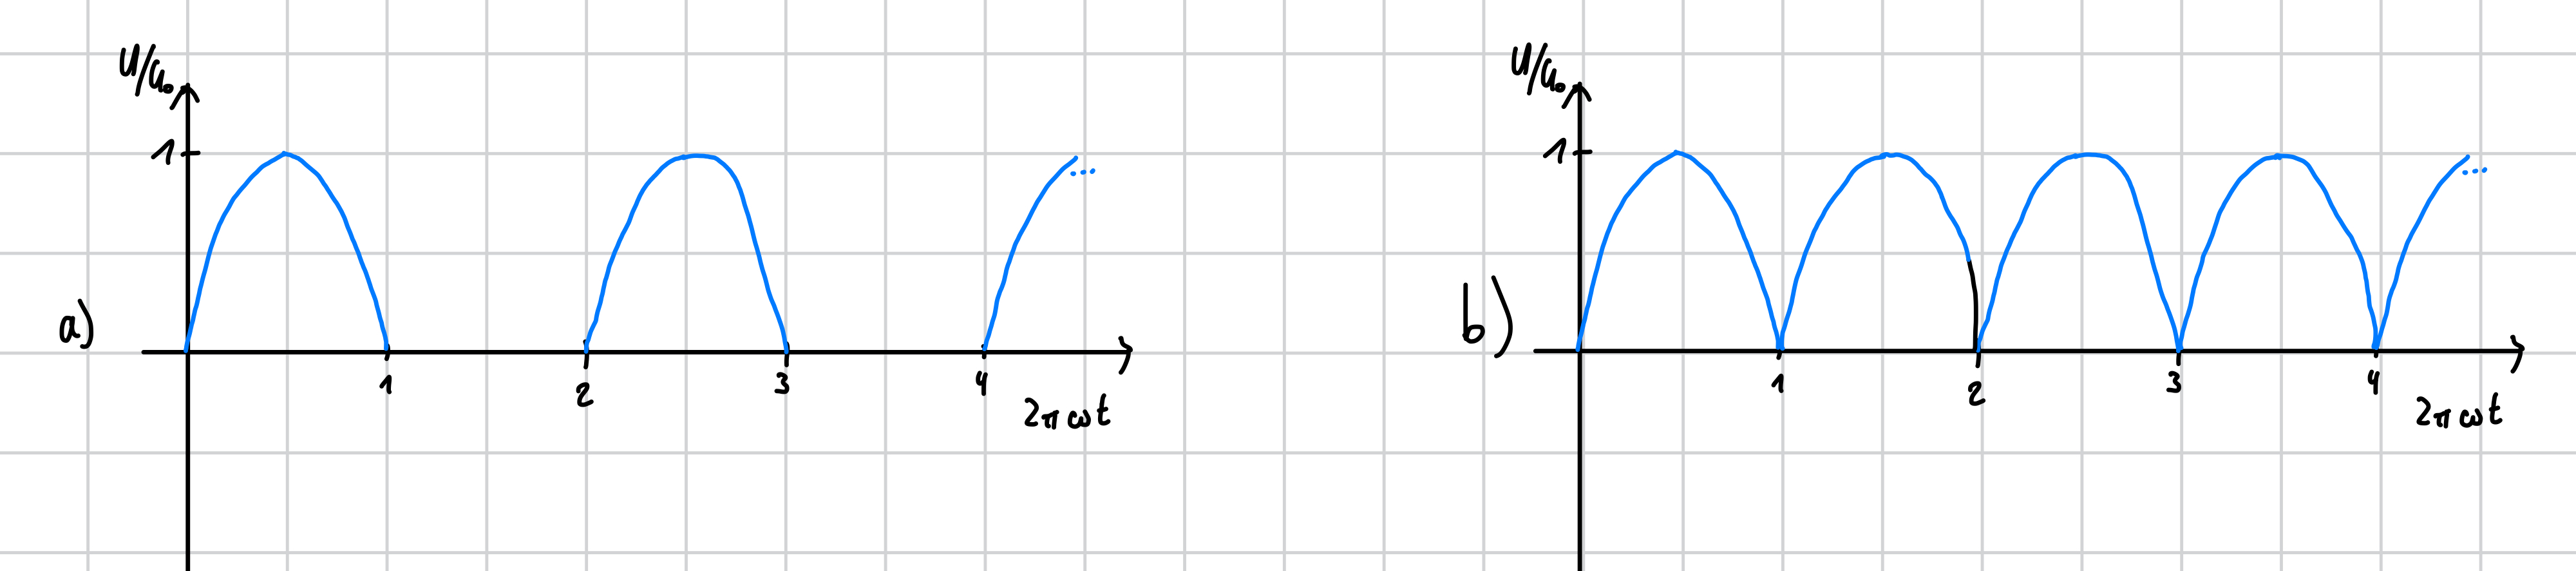
\includegraphics[width=0.8\textwidth]{figs/fig2_D.png}
        \caption{Zeitlicher Verlauf der Ausgansspannungen von Ein- und Zweiweggleichrichter}
        \label{figD}
    \end{figure}
\end{voraufgabe}
% == E ==
\begin{voraufgabe}{Wie muss $C$ dimensioniert sein, um die Welligkeit der Spannung über $R$ möglichst klein zu halten?}
Je größer die Kapazität $C$, desto länger dauert der Entladevorgang des Kondensators, was eine längere Kompensation des Brummens und somit eine stärkere Stabilisierung der Ausgansspannung zufolge hat.

\end{voraufgabe}
% == F ==
\label{F}
\begin{voraufgabe}{Wie würden Sie Strom- und Spannungsmessgerät zur Messung der Kennlinie in Durchlassrichtung und in Sperrrichtung anordnen? Berückstichtigen Sie die Innenwiderstände der beiden Geräte.}
Im Allgemeinen müssen Strommessgeräte in Reihe und Spannungsmessgeräte parallelgeschaltet werden. In Sperrichtung hat die Diode einen vergleichsweise hohen Widerstand, welcher für einen geringen Strom durch die Diode sorgt. Dieser sollte möglichst genau gemessen werden, weshalb die Spannungsmessung um die Diode und das Strommessgerät herum erfolgen sollte. Andersherum hat die Diode in Durchlassrichtung einen geringen Widerstand, was für einen hohen Strom sorgt, die Abweichung durch eine Spannungsmessung direkt an der Diode sind also eher gering, also zu bevorzugen.


\end{voraufgabe}
% == G ==
\label{G}
\begin{voraufgabe}{Wie kann man sich eine zu einem Strom proportionale Spannung herstellen?}
    Über einen ohmschen Widerstand fällt die Spannung proportional zur Stromstärke ab.
    

\end{voraufgabe}
% == H ==

\begin{voraufgabe}{Für Abb. 2.8 (\ref{fig:Abb2.8}): Berechnen Sie größenordnungsmäßig die größte Kapazität, die benutzt werden darf, ohne die Grenzwerte der Si-Diode zu überschreiten. Nehmen Sie dazu an, dass sich $U$ beim Einschalten um $\SI{1}{\volt}$ in $\SI{100}{\micro\second}$ ändert und vernachlässigen Sie den Einfluss von $R_L$.}
    \begin{figure}[H]
        \centering
        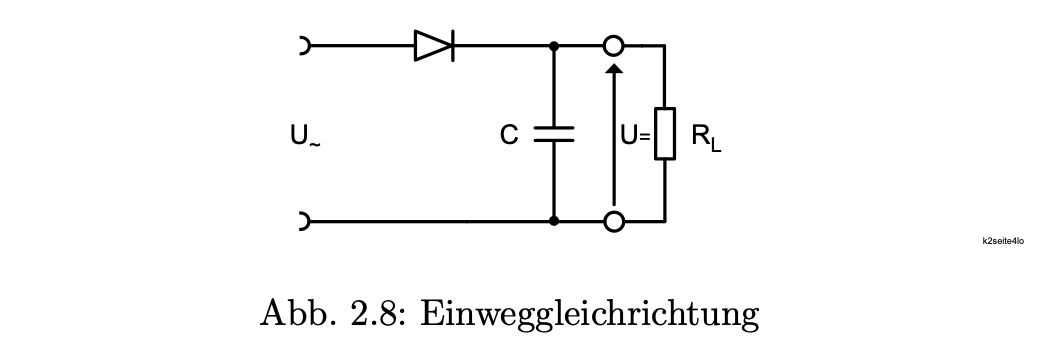
\includegraphics[width=0.8\textwidth]{figs/fig2_8.png}
        \caption{Einweggleichrichtung\cite{anleitung}}
        \label{fig:Abb2.8}
    \end{figure}
Der Maximalstrom $I_\mathrm{max}$ einer Si-Diode beträgt $\SI{1000}{\milli\ampere}$ (Seite 27 der Anleitung\cite{anleitung}). Wegen Ladungserhaltung gilt:
\begin{equation*}
    C_\mathrm{max} \Delta U = I_\mathrm{max} \Delta t
\end{equation*}
Also:
\begin{equation*}
    C_\mathrm{max} = I_\mathrm{max} \frac{\Delta t}{\Delta U} = \SI{1}{\ampere} \frac{\SI{100}{\micro\second}}{\SI{1}{\volt}} = \SI{100}{\micro\farad}
\end{equation*}
\end{voraufgabe}
% == I ==
\begin{voraufgabe}{Skizzieren Sie den zeitlichen Verlauf der Spannung am Ausgang der Schaltungen in Abb. 2.9.}
    \begin{figure}[H]
        \centering
        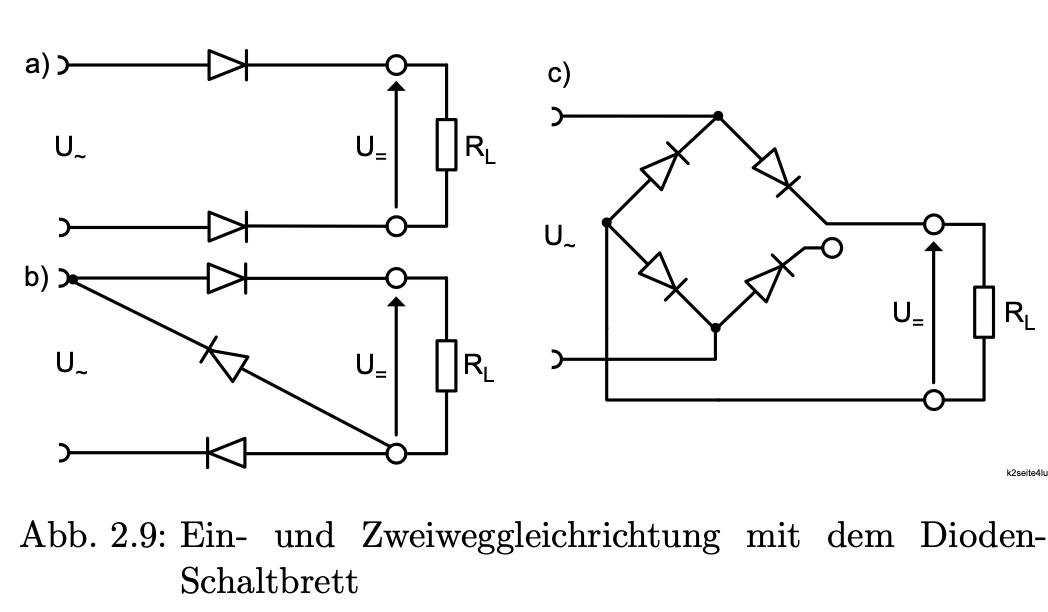
\includegraphics[width=0.8\textwidth]{figs/fig2_9.png}
        \caption{Ein- und Zweiweggleichrichtung mit dem Diodenschaltbrett\cite{anleitung}}
        \label{fig:Abb2.9}
    \end{figure}
    \begin{figure}[H]
        \centering
        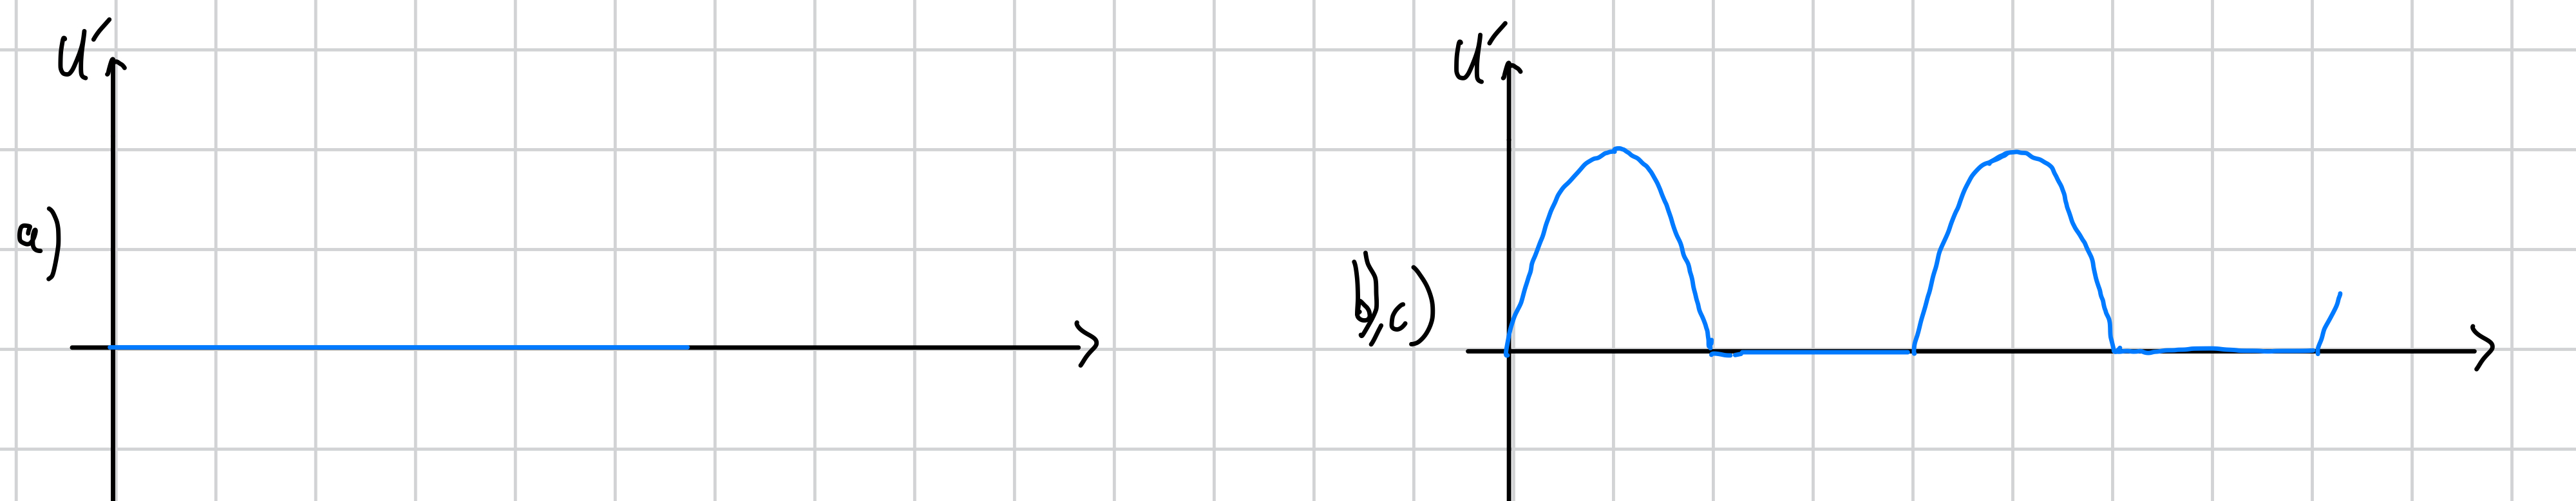
\includegraphics[width=0.8\textwidth]{figs/fig2_I.png}
        \caption{Zeitlicher Verlauf der Spannung am Ausgang der Ein- und Zweiweggleichrichtungsschaltungen}
        \label{figI}
    \end{figure}
\end{voraufgabe}
% == J ==
\begin{voraufgabe}{Skizzieren Sie die Lastabhängigkeit der Spannung $U'$ der Schaltung auf der linken Seite in Abb. 2.11. Geben Sie die Formel an, aus der sich $U'$ in Abhängigkeit von $U_0$,$R$ und $R_L$ berechnen lässt. Was sind die Extremwerte für $U'$ und $I$?}
    \begin{figure}[H]
        \centering
        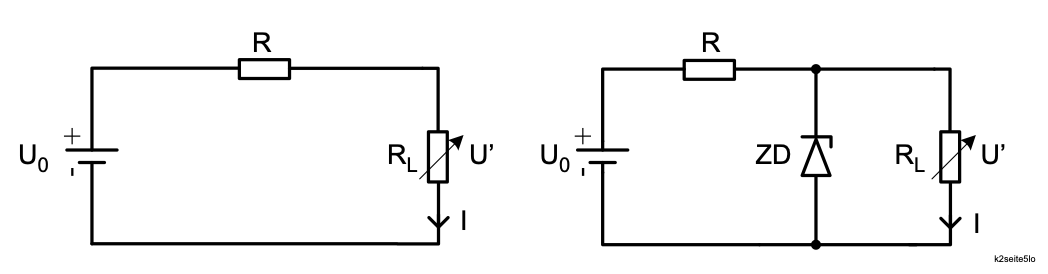
\includegraphics[width=0.8\textwidth]{figs/fig2_11.png}
        \caption{Spannungsstabilisierung mittels Zenerdiode\cite{anleitung}}
        \label{fig:Abb2.11}
    \end{figure}
    \begin{figure}[H]
        \centering
        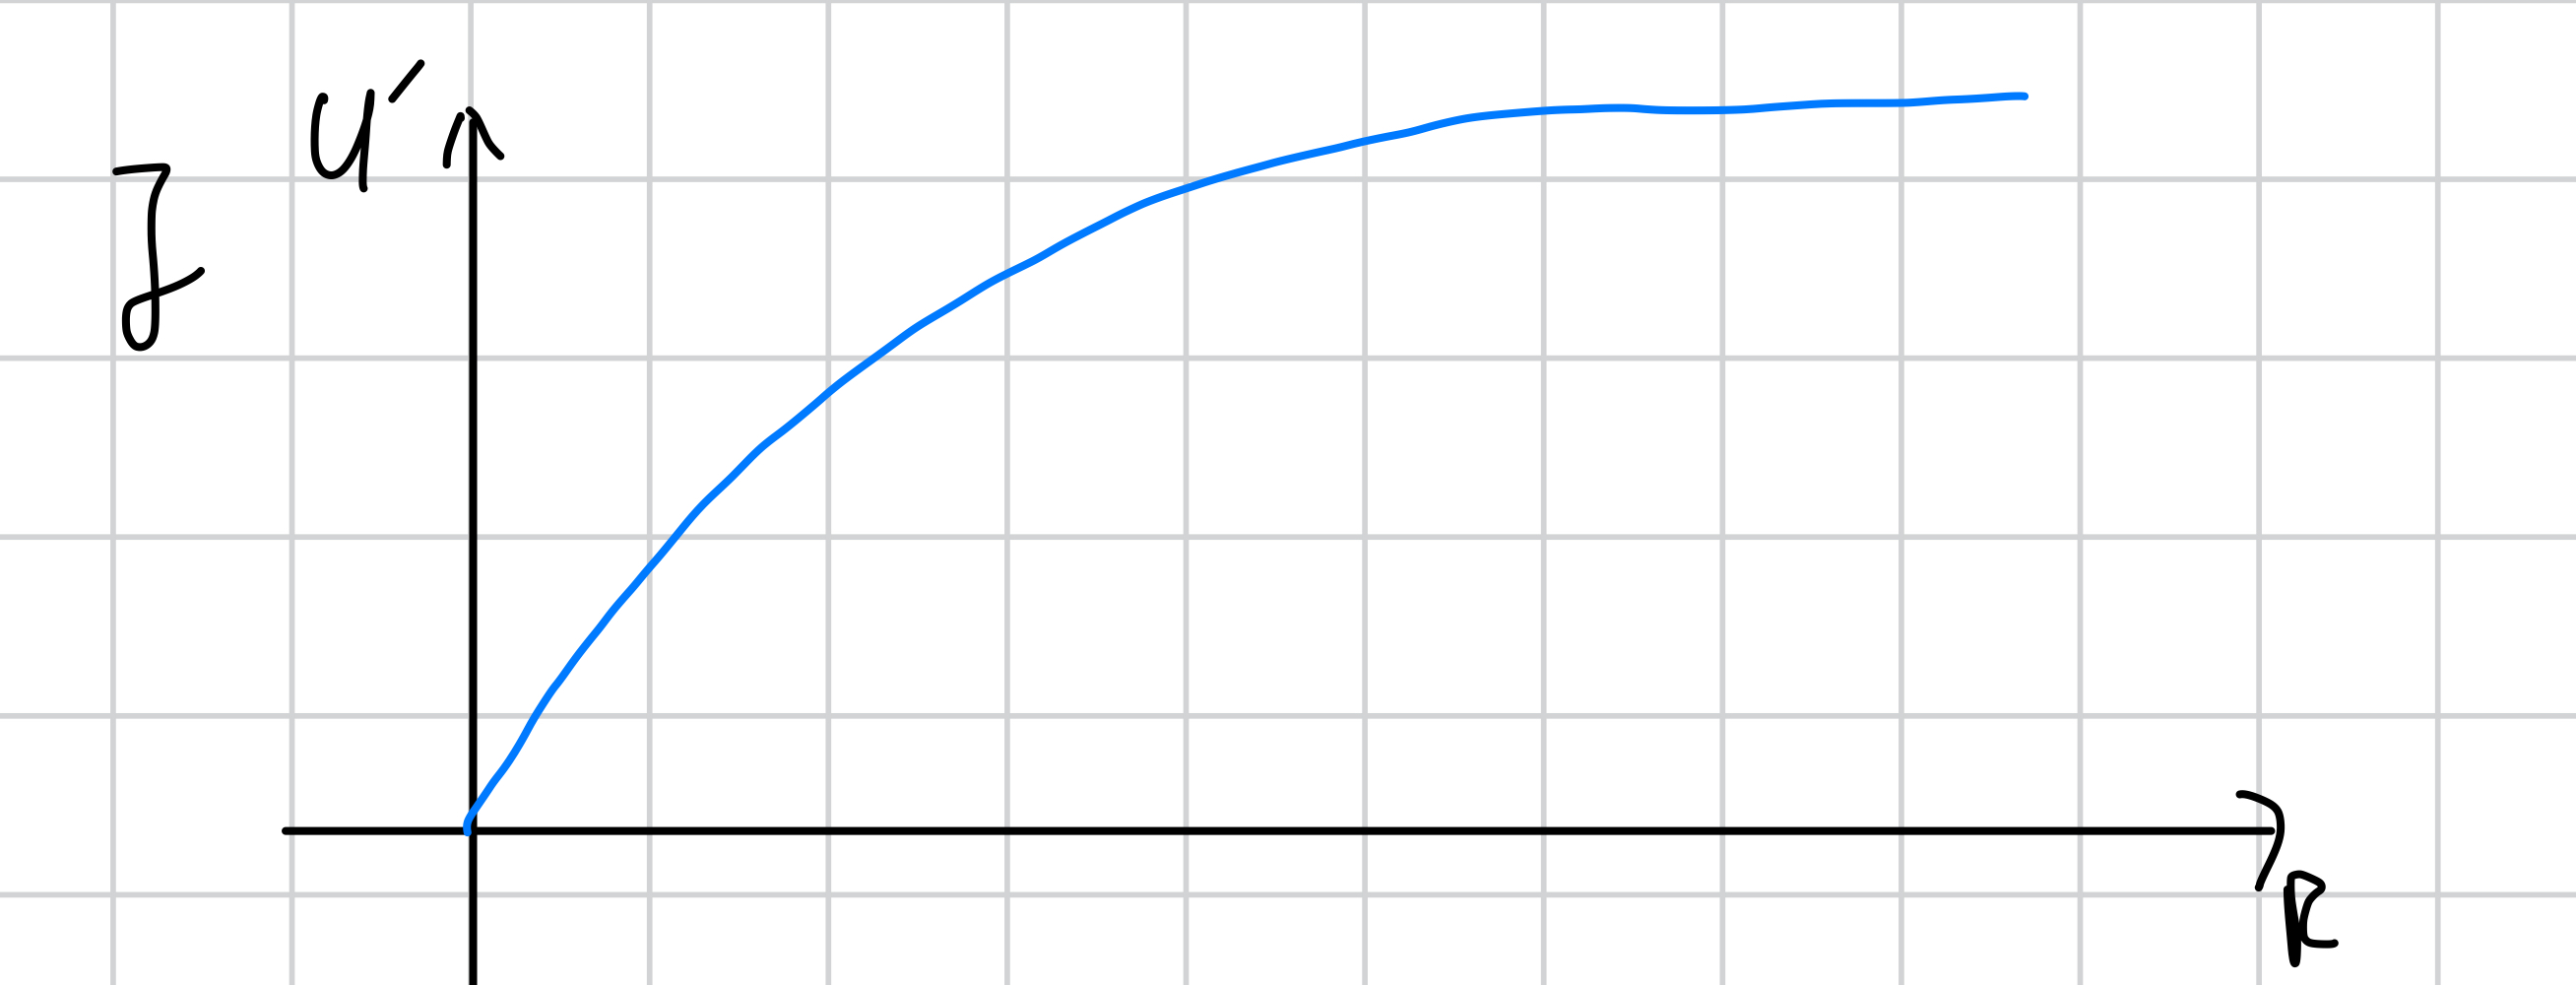
\includegraphics[width=0.8\textwidth]{figs/fig2_J.png}
        \caption{Lastabhängigkeit der Spannung $U'$}
        \label{figJ}
    \end{figure}
    Gemäß Kirchhoff gilt:
    \begin{align*}
        U_0 &= R I + R_L I\\
        U' &= I R_L
        \implies U' = U_0 \frac{R_L}{R+R_L}
    \end{align*}
    Da $R$ und $R_L$ nichtnegativ sind, gilt:
    \begin{align*}
        U_\mathrm{\max{}}' &= U_0 \\
        U_\mathrm{\min{}}' &= 0 \\
        I_\mathrm{\max{}}' &= \frac{U_0}{R} \\
        I_\mathrm{\min{}}' &= 0
    \end{align*}

\end{voraufgabe}
% == K ==
\begin{voraufgabe}{Innerhalb welches \underline{Wertebereiches} muss bei dieser Dimensionierung der Arbeitswiderstand $R$ liegen, damit die Ausgangsspannung $U'$ bei der Zenerspannung von $\SI{8.2}{\volt}$ stabilisiert wird?}
    Betriebsdaten der Zenerdiode:
    \begin{align*}
        U_\mathrm{Z}&=\SI{8.2}{\volt}\\
        U_\mathrm{0,max}&=\SI{22}{\volt}\\
        U_\mathrm{0,min}&=\SI{16}{\volt}\\
        I_\mathrm{Z,max}&=\SI{100}{\milli\ampere}\\
        I_\mathrm{Z,min}&=\SI{2}{\milli\ampere}
    \end{align*}
    Falls $R_\mathrm{L}=\infty$, läuft der gesamte Strom durch die Zenerdiode. Dieser darf $I_\mathrm{Z,max}$ nicht überschreiten. Daher muss $R_\mathrm{min}$ entsprechend gewählt werden:
    \begin{align*}
        I_\mathrm{R}&=I_\mathrm{Z,max}=\frac{U_\mathrm{0,max}-U_\mathrm{Z}}{R}\\
        \Rightarrow R&>\frac{U_\mathrm{0,max}-U_\mathrm{Z}}{I_\mathrm{Z,max}}=\SI{138}{\ohm}
    \end{align*}
    Weiterhin darf unter keinen Umständen der Wert für $I_\mathrm{Z,min}=\SI{2}{\milli\ampere}$ unterschritten werden. Hierfür muss der Fall $U_0=U_\mathrm{0,min}$ und $R_\mathrm{L}=\SI{200}{\ohm}$ betrachtet werden:
    \begin{align*}
        I_\mathrm{Z,min} &= I_\mathrm{R}-I_\mathrm{L} \\
        &= \frac{U_\mathrm{0,min}-U_\mathrm{Z}}{R}-\frac{U_\mathrm{Z}}{R_\mathrm{L,min}} \\
        \Rightarrow R &< \frac{U_\mathrm{0,min}-U_\mathrm{Z}}{I_\mathrm{Z,min}+\frac{U_\mathrm{Z}}{R_\mathrm{L,min}}} = \SI{181}{\ohm}
    \end{align*}    
\end{voraufgabe}


\clearpage
\section{Versuchsaufbau, -durchführung, Messwerte und Auswertung}
% === Aufbau, Durchführung, Messwerte und Auswertung ===
% == Aufgabe 1 ==
\begin{aufgabe}{Statische Messung der Diodenkennlinie} 
    \aufbau
    \begin{figure}[H]
        \centering
        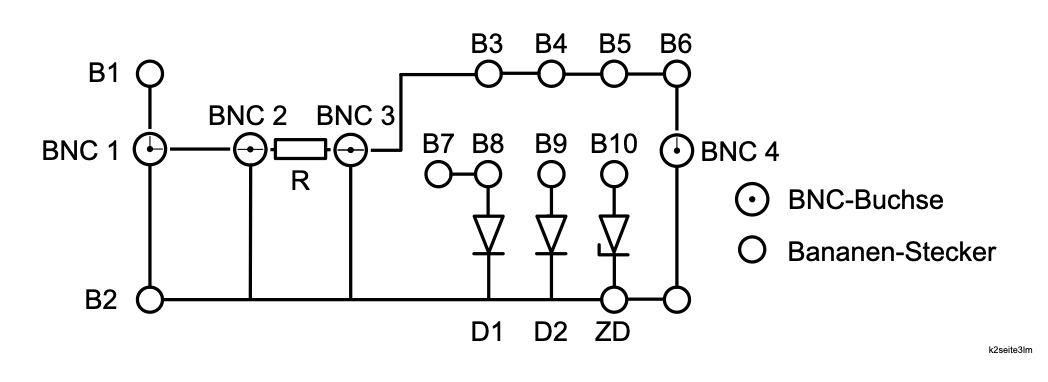
\includegraphics[width=0.8\textwidth]{figs/fig2_6.png}
        \caption{oberer Teil des Diodenschaltbretts\cite{anleitung}}
        \label{aufbau_2_1}
    \end{figure}
Zunächst soll die Diodenkennlinie der unbekannten Dioden D1 und D2 mittels einer statischen Messung ermittelt werden.
 Dafür wird entsprechend der Voraufgabe~F~(\ref{F}) mit Ampère- und Voltmeter gemessen. Die Messwerte werden dann in einer 
 Tabelle aufgelistet, wie zum Beispiel \ref{tab:D1duchlass}, \ref{tab:D1sperr}. 

\begin{table}[h!]
    \centering
    \begin{tabular}{|l|l|}
    \hline
    \textbf{Spannung $U$ in $[V]$} & \textbf{Strom $A$ in $[mA]$} \\
    \hline
    $0.104$ & $0$ \\
    $0.201$ & $0$\\
    $0.304$ &  $2 \cdot 10^-3$ \\
    $0.401$ & $2 \cdot 10^-3$\\
    $0.501$ & $0.13$ \\
    $0.601$ & $0.50$ \\
    $0.701$ & $1.1$ \\
    $0.802$ & $1.9$ \\
    $0.902$ & $2.7$ \\
    $1.003$ & $3.5$ \\
    $1.513$ & $8.5$ \\
    $2.061$ & $13.5$ \\
    $5.02$ & $41.8$ \\
    \hline
    \end{tabular}
    \caption{Kennlinie D1 in Durchlassrichtung}
    \label{tab:D1duchlass}
    \end{table}
    
    \newpage

    \begin{table}[h!]
    \centering
    \begin{tabular}{|l|l|}
    \hline
    \textbf{Spannung $U$ in $[V]$} & \textbf{Strom $A$ in $[\mu A]$} \\
    \hline
    $-1.004$ & $0$ \\
    $-2.009$ & $0$\\
    $-3.009$ & $0$\\
    $-4.002$ & $0$\\
    $-5.10$ & $0.5$\\
    $-6.04$ & $0.5$\\
    $-7.05$ & $0.8$\\
    $-8.07$ & $0.9$\\
    $-9.004$ & $1$\\
    $-10.05$ & $1$\\
    $-11.00$ & $1,1$\\
    $-12.03$ & $1.2$\\
    \hline
    \end{tabular}
    \caption{Kennlinie D1 in Sperrrichtung}
    \label{tab:D1sperr}
    \end{table}

    Nun bringt man die 2 Tabellen zusammen und erstellt man damit eine graphische Darstellung, wobei $5\%$ der ausgemessenen Werte
    gewählt wird. Die Rest der Tabellen sowie Abbildungen für den Schottky-Diode
     sind im Anhang zu finden. 
     \begin{figure}[H]
        \centering
        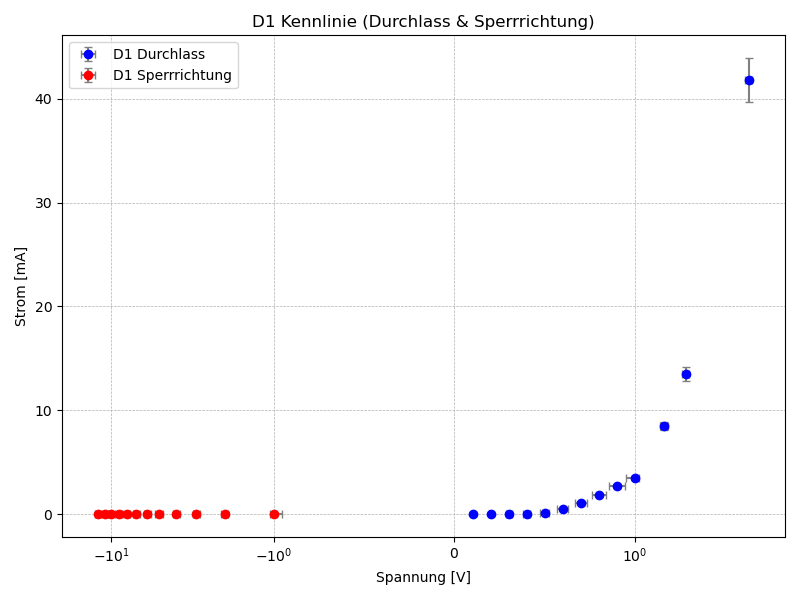
\includegraphics[width=0.8\textwidth]{figs/dioden_d1_combined.png}
        \caption{Kennlinienverlauf der Siliziumdiode in Durchlassrichtung und Sperrrichtung aus Tabellen \ref{tab:D1duchlass}, \ref{tab:D1sperr} }
        \label{dioden_d1_combined}
    \end{figure}

    \begin{figure}[H]
        \centering
        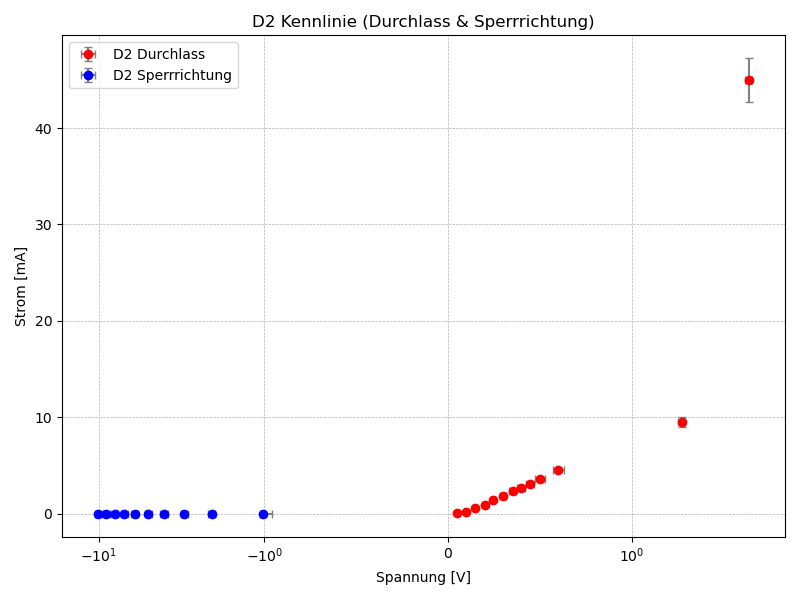
\includegraphics[width=0.8\textwidth]{figs/dioden_d2_combined.png}
        \caption{Kennlinienverlauf der Schottky-Diode in Durchlassrichtung und Sperrrichtung aus Tabellen \ref{tab:D2duchlass}, \ref{tab:D2sperr}}
        \label{dioden_d1_combined}
    \end{figure}

    
\end{aufgabe}
\newpage 
% == Aufgabe 2 ==
\begin{aufgabe}{Oszillogramm der Diodenkennlinie}
    \aufbau
    \begin{figure}[H]
        \centering
        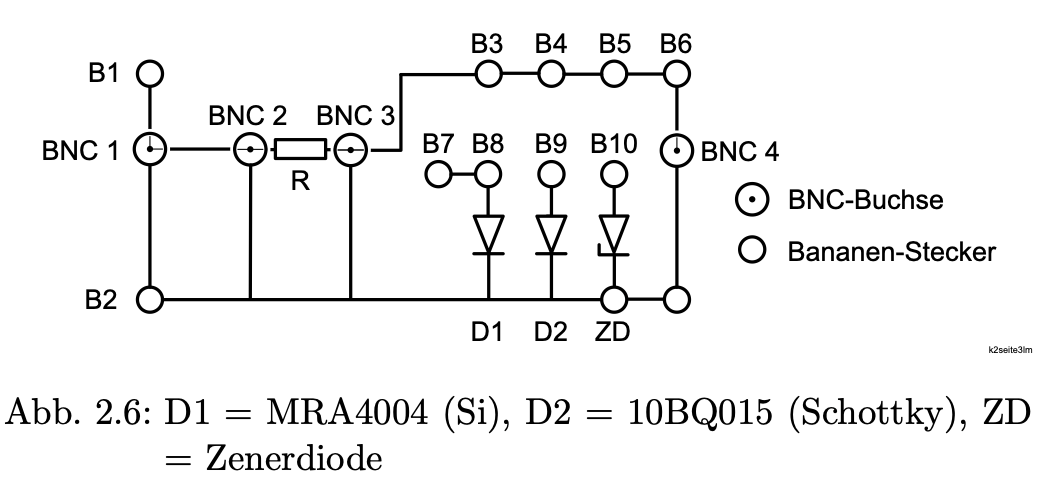
\includegraphics[width=0.8\textwidth]{figs/Aufbau2.png}
        \caption{oberer Teil des Diodenschaltbretts\cite{anleitung}}
        \label{aufbau_2_2}
    \end{figure}
Nun soll die Messung nicht mehr analog erfolgen, sondern mittels eines Oszillographens. Hierfür wird der Strom gemäß Voraufgabe~G~(\ref{G}) in eine Spannung umgewandelt und dann im Oszillographen im x-y-Modus gegen die anliegende Spannung aufgetragen. Außerdem wird das Bild auf dem Oszilloskop zentriert, indem bei einer sehr geringen Amplitude des Signalgenerators ein Punkt entsteht, der mit den Offsets des Oszillographen auf den Ursprung verschoben wird.
    \messwerte 
    \begin{figure}[H]
        \centering
        \begin{subfigure}[b]{0.45 \textwidth}
            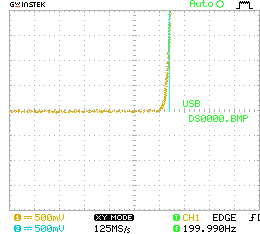
\includegraphics[width=\textwidth]{MesswerteVersuch2/m2_0.png}
            \caption{Silizium-Diode (D1)}
            \label{a2_0}
        \end{subfigure}
        \hfill
        \begin{subfigure}[b]{0.45 \textwidth}
            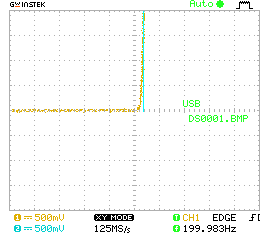
\includegraphics[width=\textwidth]{MesswerteVersuch2/m2_1.png}
            \caption{Schottky-Diode (D2)}
            \label{a2_1}
        \end{subfigure}
        \hfill
        \begin{subfigure}[b]{0.45 \textwidth}
            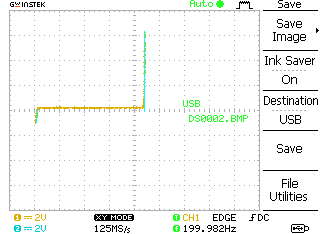
\includegraphics[width=\textwidth]{MesswerteVersuch2/m2_2.png}
            \caption{Zener-Diode (ZD)}
            \label{a2_2}
        \end{subfigure}
        \caption{Kennlinien der verschiedenen Dioden}
        \label{a2}
    \end{figure}
    \auswertung
    Aus den x-y-Graphen für die an der jeweiligen Diode anliegende Spannung und dem Strom, der die Diode durchfließt (bzw. einer dazu proportionalen Spannung)(\ref{a2}) lassen sich nun Diffusionsspannung und Zenerspannung (bei der Zenerdiode) graphisch ermitteln:
    \begin{align*}
        U_\mathrm{Diffusion, D1} &= \SI{0.7 +- 0.06}{\volt} \\
        U_\mathrm{Diffusion, D2} &= \SI{0.18 +- 0.06}{\volt} \\
        U_\mathrm{Diffusion, ZD} &= \SI{0.8 +- 0.24}{\volt} \\
        U_\mathrm{Zener, ZD} &= \SI{7.84 +- 0.24}{\volt} \\
    \end{align*}
    Bei den ersten beiden Dioden lässt sich keine Zenerspannung ermitteln, da im Experiment keine Spannung der passenden Größenordung verwendet wurde, um die Dioden nicht zu zerstören. Bei der Zenerdiode ist diese dann allerdings gut zu erkennen und liegt im von der Anleitung~\cite{anleitung} angegebenen Bereich von $\SIrange{3}{180}{\volt}$, der Literatur~\cite{zenerspannungen} zufolge könnte es sich um eine BZX55/C  gV2-Zenerdiode handeln, die eine Zenerspannung von $U_\mathrm{Zener}^\mathrm{theoretisch} = \SI{8.2}{\volt}$ besitzt.

    Für die Diffusionsspannung der Siliziumdiode entspricht der ermittelte Wert von $U_\mathrm{Diffusion, D1} = \SI{0.7 +- 0.06}{\volt}$ gerade dem Theoriewert $\SI{0.7}{\volt}$ der Anleitung~\cite{anleitung}. Die Diffusionsspannung der Schottkydiode soll der Theorie nach niedriger sein, was hier auch bestätigt wird: 
    \begin{equation*}
        U_\mathrm{Diffusion, D2} = \SI{0.18 +- 0.06}{\volt} < \SI{0.7 +- 0.06}{\volt} = U_\mathrm{Diffusion, D1}
    \end{equation*}
    
\end{aufgabe}
\clearpage
% == Aufgabe 3 ==
\begin{aufgabe}{Oszillogramm des Einweggleichrichters}
    \aufbau
    \begin{figure}[H]
        \centering
        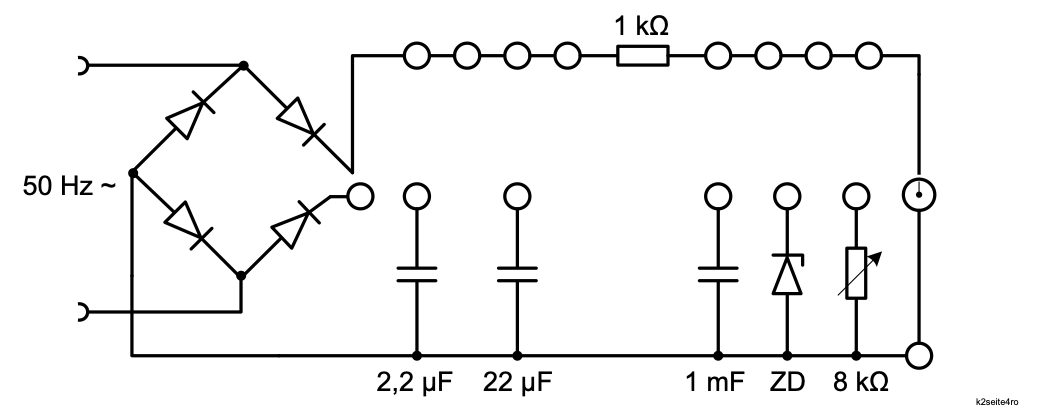
\includegraphics[width=0.8\textwidth]{figs/Aufbau3.png}
        \caption{unterer Teil des Diodenschaltbretts\cite{anleitung}}
        \label{aufbau3}
    \end{figure}
    Das Schaltbrett wird auf die Einweggleichrichtung eingestellt. Daran wird eine $\SI{50}{\hertz}$ Wechselspannung eingestellt. Als Verbraucher dient das Oszilloskop, welches die zeitliche Spannungsänderung darstellt. Zum Glätten der gleichgerichteten Spannung werden vier verschiedene Kapazitäten dem Verbraucher parallelgeschaltet.
    \messwerte
    \begin{figure}[H]
        \begin{subfigure}[b]{0.49 \textwidth}
            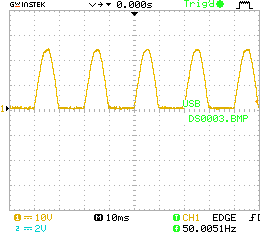
\includegraphics[width=\textwidth]{MesswerteVersuch2/DS0003.png}
            \caption{keine Glättung}
            \label{a3_a}
        \end{subfigure}
        \hfill
        \begin{subfigure}[b]{0.49 \textwidth}
            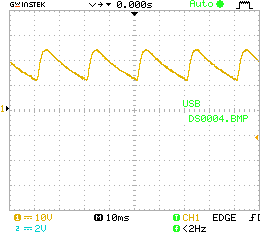
\includegraphics[width=\textwidth]{MesswerteVersuch2/DS0004.png}
            \caption{Glättung mit $C = \SI{2.2}{\micro\farad}$}
            \label{a3_b}
        \end{subfigure}
        \vspace{1em}
        \begin{subfigure}[b]{0.49 \textwidth}
            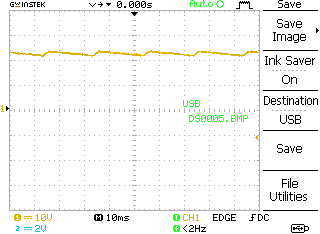
\includegraphics[width=\textwidth]{MesswerteVersuch2/DS0005.png}
            \caption{Glättung mit $C = \SI{22}{\micro\farad}$}
            \label{a3_c}
        \end{subfigure}
        \hfill
        \begin{subfigure}[b]{0.49 \textwidth}
            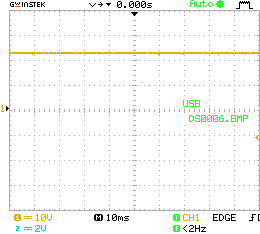
\includegraphics[width=\textwidth]{MesswerteVersuch2/DS0006.png}
            \caption{Glättung mit $C = \SI{1000}{\micro\farad}$}
            \label{a3_d}
        \end{subfigure}
        \caption{Verschiedene Glättungen eines einweggleichgerichteten Signals}
        \label{a3}
    \end{figure}
    Die mittlere Höhe der Gleichspannung und die Brumm-Amplitude werden dem Oszillographen direkt entnommen:
    \begin{table}[H]
        \centering
        \begin{tabular}{|l|l|l|l|}
            \hline
            Schaltung & Glättkapazität & mittlere Höhe der Gleichspannung & Brumm-Amplitude  \\
            \hline
            a) & $\SI{0}{\micro\farad}$ & $\SI{7.7}{\volt}$ & $\SI{24}{\volt}$ \\
            b) & $\SI{2.2}{\micro\farad}$ & $\SI{17.6}{\volt}$ & $\SI{12.6}{\volt}$ \\
            c) & $\SI{22}{\micro\farad}$ & $\SI{22.3}{\volt}$ & $\SI{2.2}{\volt}$ \\
            d) & $\SI{1000}{\micro\farad}$ & $\SI{22.4}{\volt}$ & $\SI{0.8}{\volt}$ \\
            \hline
        \end{tabular}
        \caption{Brumm- und mittlere Spannung nach Glättung}
    \end{table}
    \auswertung
    In den Grafiken~\ref{a3} kann man die Änderung des Signals für verschiedene Kapazitäten erkennen. In \ref{a3_a} ist keine Kapazität zum Glätten zwischengeschaltet, also ist das in \ref{figI} theoretisch bestimmte Bild ersichtlich. Die Brummspannung ist hier maximal und entspricht gerade der Amplitude von $\SI{24}{\volt}$. Der Mittelwert liegt deutlich unter der Amplitude, er sollte in der Theorie $\frac{\sqrt{2}}{4} U_\mathrm{Amplitude}$ entsprechen, was mit $\frac{\sqrt{2}}{4} \SI{24}{\volt} \approx \SI{8.5}{\volt}$ im Vergleich zum gemessenen Wert $\SI{7.7}{\volt}$ grob der Fall ist.

    Beim Einschalten der Kapazitäten lässt sich eine immer stärkere Glättung feststellen, einerseits in der Kurve, die immer glatter wird, andererseits in der kleiner werdenden Brumm-Amlplitude und im Steigen der mittleren Höhe der Gleichspannung.
\end{aufgabe}

\clearpage
% == Aufgabe 4 ==
\begin{aufgabe}{Oszillogramm des Zweiweggleichrichters}
    \aufbau
    \begin{figure}[H]
        \centering
        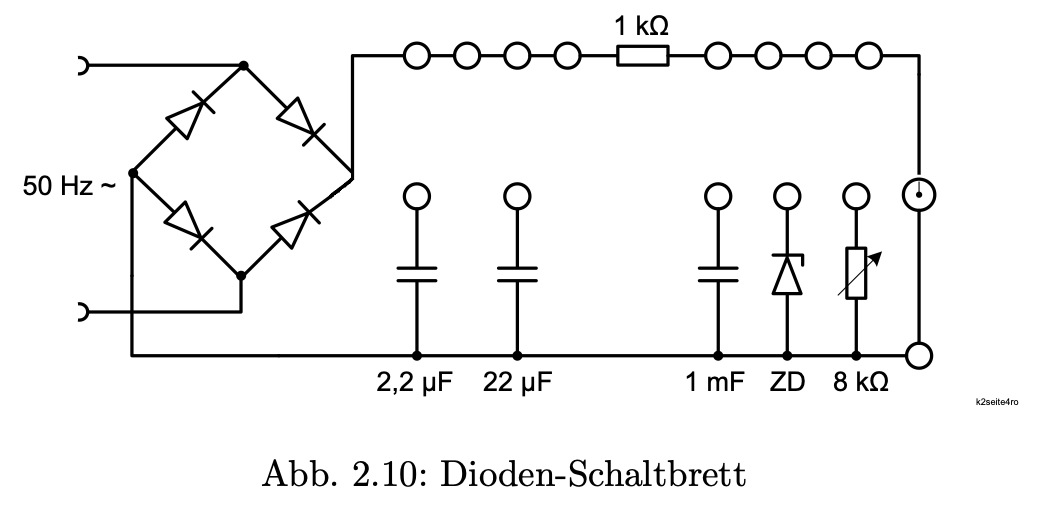
\includegraphics[width=0.8\textwidth]{figs/Aufbau4.png}
        \caption{unterer Teil des Diodenschaltbretts\cite{anleitung}}
        \label{aufbau4}
    \end{figure}
    Es wird genauso vorgegangen, wie im Einweggleichrichtungsversuchsteil, nur wird der rückläufige Gleichrichtungsweg eingeschaltet.
    \messwerte
    \begin{figure}[H]
        \begin{subfigure}[b]{0.49 \textwidth}
            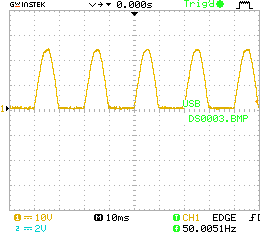
\includegraphics[width=\textwidth]{MesswerteVersuch2/DS0003.png}
            \caption{keine Glättung}
            \label{a3_a}
        \end{subfigure}
        \hfill
        \begin{subfigure}[b]{0.49 \textwidth}
            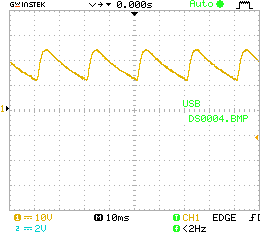
\includegraphics[width=\textwidth]{MesswerteVersuch2/DS0004.png}
            \caption{Glättung mit $C = \SI{2.2}{\micro\farad}$}
            \label{a3_b}
        \end{subfigure}
        \vspace{1em}
        \begin{subfigure}[b]{0.49 \textwidth}
            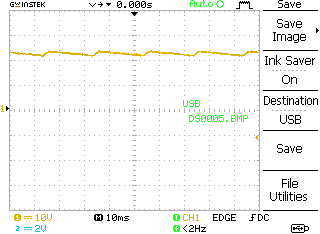
\includegraphics[width=\textwidth]{MesswerteVersuch2/DS0005.png}
            \caption{Glättung mit $C = \SI{22}{\micro\farad}$}
            \label{a3_c}
        \end{subfigure}
        \hfill
        \begin{subfigure}[b]{0.49 \textwidth}
            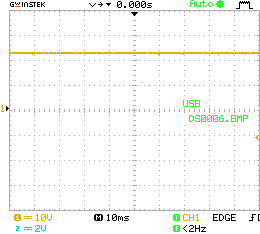
\includegraphics[width=\textwidth]{MesswerteVersuch2/DS0006.png}
            \caption{Glättung mit $C = \SI{1000}{\micro\farad}$}
            \label{a3_d}
        \end{subfigure}
        \caption{Verschiedene Glättungen eines zweiweggleichgerichteten Signals}
    \end{figure}
    \begin{table}[H]
        \centering
        \begin{tabular}{|l|l|l|l|}
            \hline
            Schaltung & Glättkapazität & mittlere Höhe der Gleichspannung & Brumm-Amplitude  \\
            \hline
            a) & $\SI{0}{\micro\farad}$ & $\SI{15}{\volt}$ & $\SI{24}{\volt}$ \\
            b) & $\SI{2.2}{\micro\farad}$ & $\SI{21}{\volt}$ & $\SI{6.8}{\volt}$ \\
            c) & $\SI{22}{\micro\farad}$ & $\SI{23}{\volt}$ & $\SI{1.3}{\volt}$ \\
            d) & $\SI{1000}{\micro\farad}$ & $\SI{23.1}{\volt}$ & $\SI{1}{\volt}$ \\
            \hline
        \end{tabular}
        \caption{Brumm- und mittlere Spannung nach Glättung}
    \end{table}
    \auswertung
    Qualitativ verhalten sich die Glättungen gleich zu denen der Einweggleichrichtung. Im Fall ohne Glättkapazität wird allerdings die mittlere Höhe der Gleichspannung verdoppelt, da hier doppelt so viele Peaks durch die Zweigweggleichrichtung entstehen: $\frac{\SI{15}{\volt}}{\SI{7.7}{\volt}} \approx 2$. Die Brummamplitude ist für jede Kapazität innerhalb einer Messungenauigkeit von $\SI{0.5}{\volt}$ kleiner als die bei der Einweggleichrichtung, was dadurch erklärt werden kann, dass die Spannung im Fall der Zweigweggleichrichtung schon "glatter" ist. Bei der stärksten Glättung ist dieser Unterschied allerdings fast schon vernachlässigbar bzw. gar nicht vorhanden, da die Glättung insgesamt stark genug ist. 

    Zusammenfassend lässt sich sagen, dass der Zweiweggleichrichter für geringe Glättkapazitäten besser glättet, als der Einweggleichrichter, dieser Effekt aber mit zunehmenden Kapazitäten abklingt. Im Zweigwegefall sind vier Dioden nötig, bei Einweggleichrichtung reicht eine einzige, also muss für die Bevorzugung einer der Methoden die Kosten der Dioden im Verhältnis zu größeren Kapazitäten untersucht werden.

\end{aufgabe}
\clearpage
% == Aufgabe 5 ==
\begin{aufgabe}{Oszillogramm des Einweggleichrichters}
    \begin{figure}[H]
        \centering
        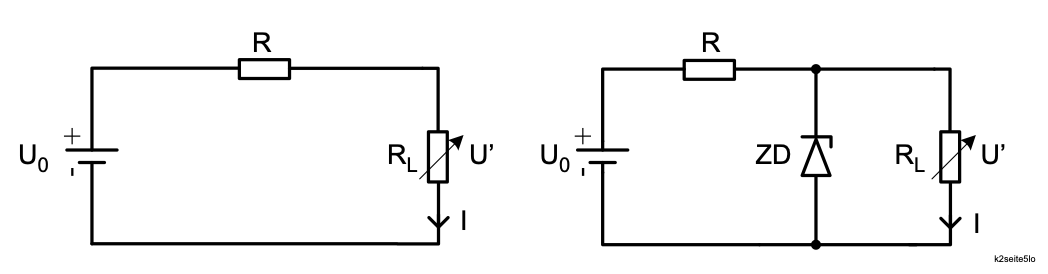
\includegraphics[width=0.8\textwidth]{figs/fig2_11.png}
        \caption{Spannungsstabilisierung mittels Zenerdiode~\cite{anleitung}}
        \label{aufbau_2_3}
    \end{figure}
\end{aufgabe}


% === Fazit ===
\section{Fazit}

% === Anhang ===%
\section{Anhang}

    
\begin{table}[h!]
    \centering
    \begin{tabular}{|l|l|}
    \hline
    \textbf{Spannung $U$ in $[V]$} & \textbf{Strom $A$ in $[mA]$} \\
    \hline
    $0.050$ & $0.02$ \\
    $0.100$ & $0.14$ \\
    $0.150$ & $0.59$ \\
    $0.200$ & $0.94$\\
    $0.247$ & $1.4$ \\
    $0.299$ & $1.8$ \\
    $0.352$ & $2.3$ \\
    $0.398$ & $2.7$\\
    $0.448$ & $3.1$ \\
    $0.502$ & $3.6$ \\
    $0.600$ & $4.5$ \\
    $2.016$ & $9.5$ \\
    $5.100$ & $45.0$ \\
    \hline
    \end{tabular}
    \caption{Kennlinie D2 in Durchlassrichtung}
    \label{tab:D2duchlass}
    \end{table}
    
    
    \begin{table}[h!]
    \centering
    \begin{tabular}{|l|l|}
    \hline
    \textbf{Spannung $U$ in $[V]$} & \textbf{Strom $A$ in $[\mu A]$} \\
    \hline
    $-1.010$ & $23$ \\
    $-2.074$ & $29$\\
    $-3.042$ & $32$\\
    $-4.03$ & $38$\\
    $-5.02$ & $43$\\
    $-6.07$ & $48$\\
    $-7.01$ & $55$\\
    $-8.01$ & $60$\\
    $-9.02$ & $65$\\
    $-10.04$ & $70$\\ 
    \hline
    \end{tabular}
    \caption{Kennlinie D2 in Sperrrichtung}
    \label{tab:D2sperr}
    \end{table}


\begin{figure}[H]
    \centering
    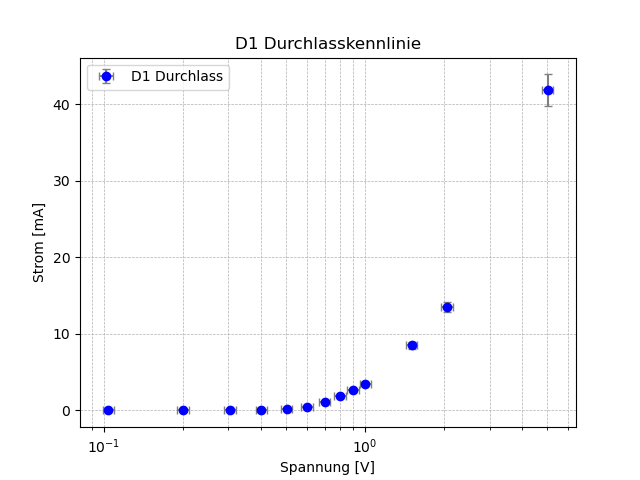
\includegraphics[width=0.8\textwidth]{figs/dioden_d1.png}
    \caption{Kennlinienverlauf der Siliziumdiode in Durchlassrichtung MRA4004; Sperrspannung 400V\cite{anleitung} }
    \label{dioden_d1}
\end{figure}

\begin{figure}[H]
    \centering
    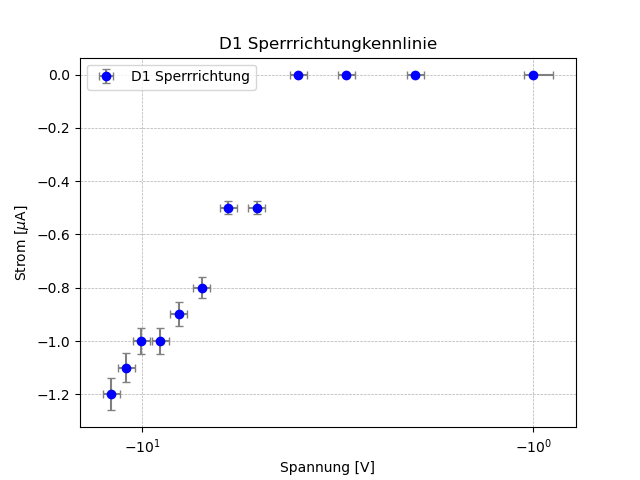
\includegraphics[width=0.8\textwidth]{figs/dioden_d1_sperr.png}
    \caption{Kennlinienverlauf der Siliziumdiode in Sperrrichtung MRA4004; Sperrspannung 400V\cite{anleitung}}
    \label{dioden_d1_sperr}
\end{figure}

\begin{figure}[H]
    \centering
    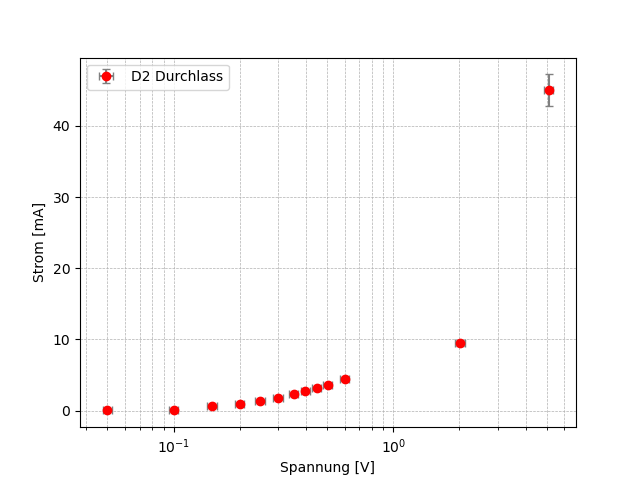
\includegraphics[width=0.8\textwidth]{figs/dioden_d2.png}
    \caption{Kennlinienverlauf der Schottky-Diode in Durchlassrichtung 10BQ015; Sperrspannung 15V\cite{anleitung}}
    \label{dioden_d2}
\end{figure}

\begin{figure}[H]
    \centering
    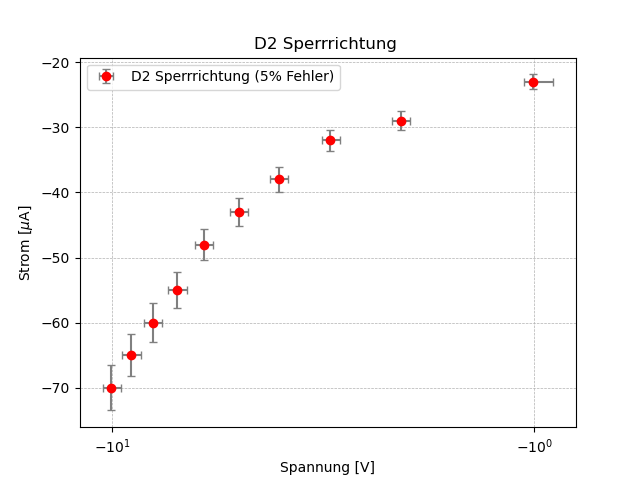
\includegraphics[width=0.8\textwidth]{figs/dioden_d2_sperr.png}
    \caption{Kennlinienverlauf der Schottky-Diode in Durchlassrichtung 10BQ015; Sperrspannung 15V\cite{anleitung}}
    \label{dioden_d2_sperr}
\end{figure}

\clearpage
% === Abbildungsverzeichnis ===
\listoffigures
% === Literaturverzeichnis
\printbibliography

\end{document}